\documentclass{beamer}

\usepackage{listings}
\usepackage{xcolor}
\usepackage{multicol}
\usepackage{amsmath}
\usepackage{hyperref}
\usepackage{comment}

\setbeamertemplate{navigation symbols}{}
\setbeamertemplate{footline}[frame number]


% Dark mode
%\begin{comment}
\definecolor{fontColor}{rgb}{1,1,1}
\definecolor{backgroundColor}{rgb}{0,0,0}
\definecolor{titleColor}{rgb}{1,0.4,0.4} % #FF6666 RGB(255, 102, 102)
\definecolor{linkColor}{rgb}{1,0.8,0.4} % #FFCC66 RGB(255, 204, 102)
\logo{
\includegraphics[height=1.5cm]{imgs/Logo_CPCFI_black}}
%\end{comment}

% Light mode
\begin{comment}
\definecolor{fontColor}{rgb}{0,0,0}
\definecolor{backgroundColor}{rgb}{1,1,1}
\definecolor{titleColor}{rgb}{0.94,0.14,0.24} % #EF233C RGB(239, 35, 60)
\definecolor{linkColor}{rgb}{1,0.6,0} % #FF9900 RGB(255, 153, 0)
\logo{
\includegraphics[height=1.5cm]{imgs/Logo_CPCFI_white}}
\end{comment}



\setbeamercolor{normal text}{fg=fontColor}
\setbeamercolor{background canvas}{bg=backgroundColor}
\setbeamercolor{title}{fg=titleColor}
\setbeamercolor{frametitle}{fg=titleColor}


\setbeamercolor{section in head/foot}{bg=titleColor}
\setbeamercolor{author in head/foot}{bg=titleColor}
\setbeamercolor{date in head/foot}{fg=titleColor}

\setbeamercolor{item}{fg=linkColor}
\setbeamercolor{caption name}{fg=linkColor}


\setbeamercolor{bibliography item}{fg=linkColor}
\setbeamercolor{bibliography entry author}{fg=linkColor}
\setbeamercolor{bibliography entry title}{fg=linkColor}
\setbeamercolor{bibliography entry location}{fg=linkColor}
\setbeamercolor{bibliography entry note}{fg=linkColor}


\definecolor{codegreen}{rgb}{0,0.6,0}
\definecolor{codegray}{rgb}{0.5,0.5,0.5}
\definecolor{codepurple}{rgb}{0.58,0,0.82}
\definecolor{backcolour}{rgb}{0.95,0.95,0.92}

\lstdefinestyle{mystyle}{
    backgroundcolor=\color{backgroundColor},
    commentstyle=\color{codegreen},
    keywordstyle=\color{magenta},
    numberstyle=\tiny\color{codegray},
    stringstyle=\color{codepurple},
    basicstyle=\ttfamily\footnotesize,
    breakatwhitespace=false,         
    breaklines=true,                 
    captionpos=b,                    
    keepspaces=true,                 
    numbers=left,                    
    numbersep=5pt,                  
    showspaces=false,                
    showstringspaces=false,
    showtabs=false,                  
    tabsize=2
}
\lstset{style=mystyle}
\hypersetup{
    colorlinks=true,
    linkcolor=linkColor,
    filecolor=magenta,      
    urlcolor=cyan
}
\urlstyle{same}

%---------------------------------------------------------------------------------------------
%---------------------------------------------------------------------------------------------
%---------------------------------------------------------------------------------------------
\title{6: Graph I}
\author{CPCFI}
\institute{UNAM's School of Engineering}
\date{2021 \\ \vspace{0.5cm} \scriptsize{Based on: Halim S., Halim F.\textit{Competitive Programming 3}}. Handbook for ACM ICPC and IOI Contestants. 2013}

\begin{document}

\frame{\titlepage}

\AtBeginSection[]
{
  \begin{frame}
    \frametitle{Table of Contents}
    \tableofcontents[currentsection]
  \end{frame}
}

%---------------------------------------------------------------------------------------------
%---------------------------------------------------------------------------------------------
%---------------------------------------------------------------------------------------------
\section{4.2 Graph Traversal}

\begin{frame}[fragile]
\frametitle{Graph Traversal - Motivation}

\begin{itemize}
    \item At least one graph problem in ICPC
    \item We should be familiar with the following concepts:
\end{itemize}

\vspace{0.3cm}

\begin{figure}
    \centering
    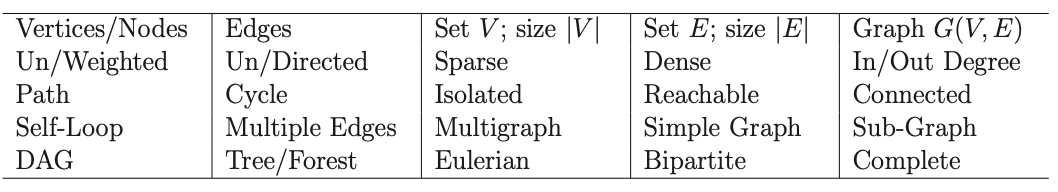
\includegraphics[scale=0.5]{imgs/important_graph_terminologies.png}
\end{figure}

\end{frame}

\begin{frame}[fragile]
\frametitle{Graph Traversal}

Topics to cover:

\begin{itemize}
    \item Depth First Search (DFS)
    \item Breadth First Search (BFS)
    \item Finding Connected Components (Undirected graph)
    \item Flodd Fill - Labeling/Coloring the Connected Components
    \item Topological Sort (DAG)
    \item Bipartite Graph Check
    \item Graph Edges Property Check via DFS Spanning Tree
    \item Finding Articulation Points and Bridges
    \item Finding Strongly Connected Components
\end{itemize}
  
\end{frame}


\begin{frame}[fragile]
\frametitle{DFS - Depth First Search}

\begin{itemize}
    \item Depth First Search is an algorithm from traversing a graph
    \item DFS visits all the reachable nodes starting from a vertex $v$
\end{itemize}

\vspace{0.3cm}

Steps:

\begin{enumerate}
    \item DFS starts from a source vertex $v$ and starts going deeper into the graph until reaching a leaf node
    \item Once DFS is on a leaf node, DFS will backtrack and explore other unvisited neighbors if any
\end{enumerate}

\end{frame}

\begin{frame}[fragile]
\frametitle{DFS}

\begin{lstlisting}[language=c]
#define MAX_N 10000
vector<int> adjList[MAX_N];
vector<int> visited(MAX_N);

void dfs(int u) {
	visited[u] = 1;
	for(auto v : adjList[u]) {
		if (visited[v] == 0) {
			dfs(v);
		}
	}
}

\end{lstlisting}

\end{frame}

\begin{frame}[fragile]
\frametitle{DFS}

\begin{itemize}
    \item DFS runs in $O(V+E)$ time
\end{itemize}

\end{frame}


\begin{frame}[fragile]
\frametitle{BFS - Breadth First Search}

\begin{itemize}
    \item BFS will traverse the graph by expanding, first, all of the neighbors starting from vertex $v$
	\item BFS uses a queue to keep track of the vertices to visit next
	\item BFS also runs in $O(V+E)$ time
\end{itemize}

\end{frame}

\begin{frame}[fragile]
\frametitle{BFS}

\begin{lstlisting}[language=c]
queue<int> q;

void bfs(int u) {
	q.push(u);
	while (!q.empty()) {
		int v = q.top(); q.pop();
		for (auto x : adjList[v]) {
			q.push(x);
		}
	}
}
\end{lstlisting}

\end{frame}

\begin{frame}[fragile]
\frametitle{Finding Connected Components - Undirected Graph}

\begin{itemize}
    \item Both DFS and BFS can also be applied to other problems
    \item A single call of DFS or BFS will visit vertices that are connected to a starting vertex $u$ in an undirected graph
\end{itemize}

\begin{figure}[H]
    \centering
    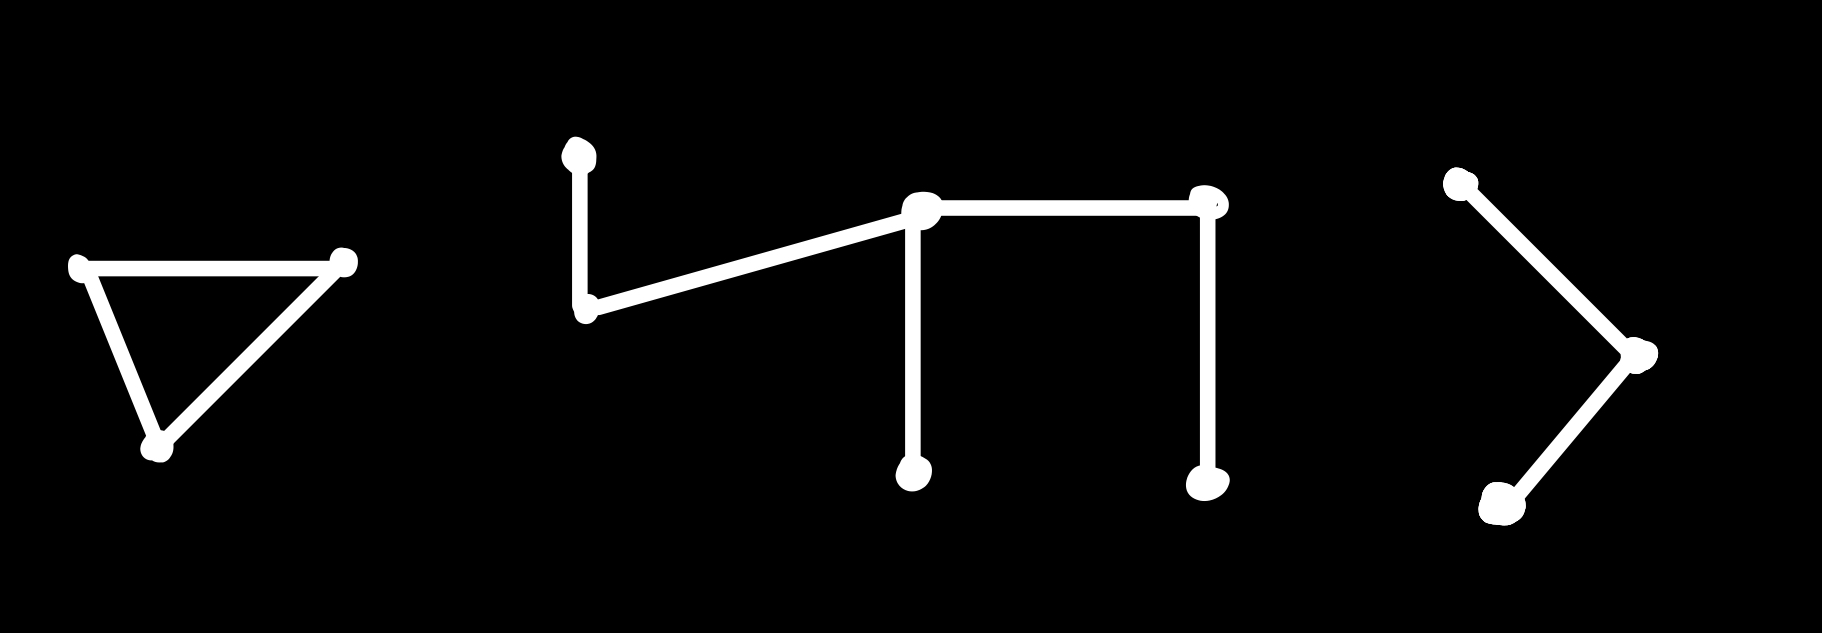
\includegraphics[scale=0.1]{imgs/non_connected_graph.jpeg}
    \caption{Undirected graph with 3 connected components}
\end{figure}

\end{frame}

\begin{frame}[fragile]
\frametitle{Finding Connected Components - Undirected Graph}

\begin{itemize}
    \item To find the number of connected components in an undirected graph iterate over all vertices
    \item For each vertex, run \textbf{dfs} if that vertex is unvisited
    \item Increase the count of connected components for each iteration over the vertices
\end{itemize}

\end{frame}

\begin{frame}[fragile]
\frametitle{Flood Fill - Labeling/Coloring the Connected Components}

\begin{itemize}
    \item Graph traversal can also be used to label a graph (color it)
    \item Or, counting the size of a connected component
    \pause
    \item Counting the size of a connected component is referred as \textbf{flood fill}
\end{itemize}

\vspace{1cm}

\textbf{Example:} \href{https://onlinejudge.org/index.php?option=com_onlinejudge&Itemid=8&category=6&page=show_problem&problem=410}{UVa 469 - Wetlands of Florida}

\end{frame}

\begin{frame}[fragile]
\frametitle{Topological Sort - Directed Acyclic Graph}

\begin{itemize}
    \item The topological sort of a DAG is a linear ordering of the vertices so that vertex $u$ comes before vertex $v$ if edge $u \rightarrow v$ exists
  	\pause
	\item Every DAG has at least one topological sort
\end{itemize}

\end{frame}

\begin{frame}[fragile]
\frametitle{Topological Sort - Directed Acyclic Graph}

\begin{figure}[H]
    \centering
    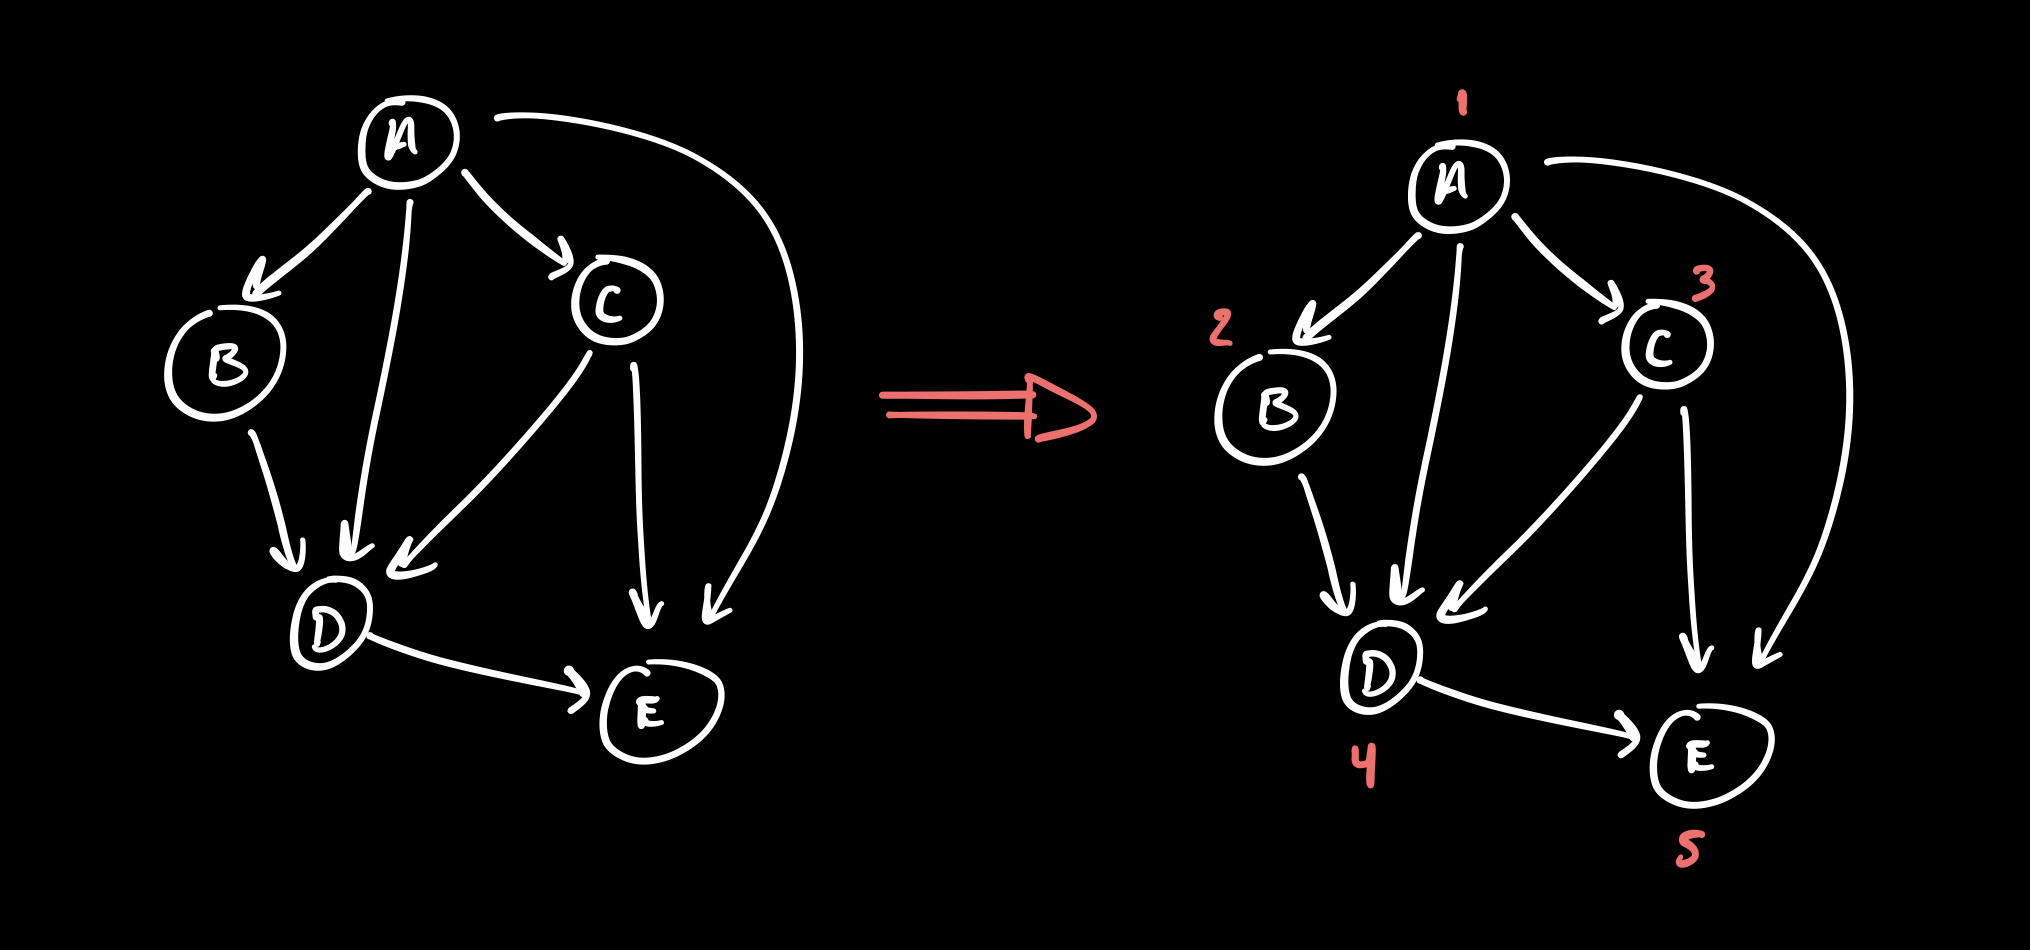
\includegraphics[scale=0.15]{imgs/topological_sort.jpeg}
    \caption{Example of a Topological Sort for a DAG}
\end{figure}

\end{frame}

\begin{frame}[fragile]
\frametitle{Topological Sort - Directed Acyclic Graph}

\begin{itemize}
    \item One common application of Topological Sort is to find a sort upcoming tasks in order of precedence
    \item For example, ordering the steps needed to cook pizza. Each step needs a previous step to be completed (mass, tomatoes, etc)
\end{itemize}

\end{frame}

\begin{frame}[fragile]
\frametitle{Topological Sort - Directed Acyclic Graph}

\begin{itemize}
    \item Topological Sort can be achieved by appending the current visited node in DFS -after visiting all the nodes in its subtree- to a list
\end{itemize}

\pause

\begin{lstlisting}[language=c]
vector<int> topological_sort;

void dfs(int u) {
	visited[u] = 1;
	for (auto v : adjList[u]) {
		if (visited[v] == 0) {
			dfs(v);
		}
	}
	// Only change for TS
	topological_sort.push_back(u);
}
\end{lstlisting}

\end{frame}

\begin{frame}[fragile]
\frametitle{Bipartite Graph Check}

\begin{itemize}
    \item A graph is said to be bipartite if its 2-colorable
    \item Thus, we'll check if a graph is bipartite by attempting to color it only 2 colors
    \item We'll achieve this by modifying BFS
\end{itemize}

\end{frame}

\begin{frame}[fragile]
\frametitle{Bipartite Graph Check}

\begin{figure}[H]
    \centering
    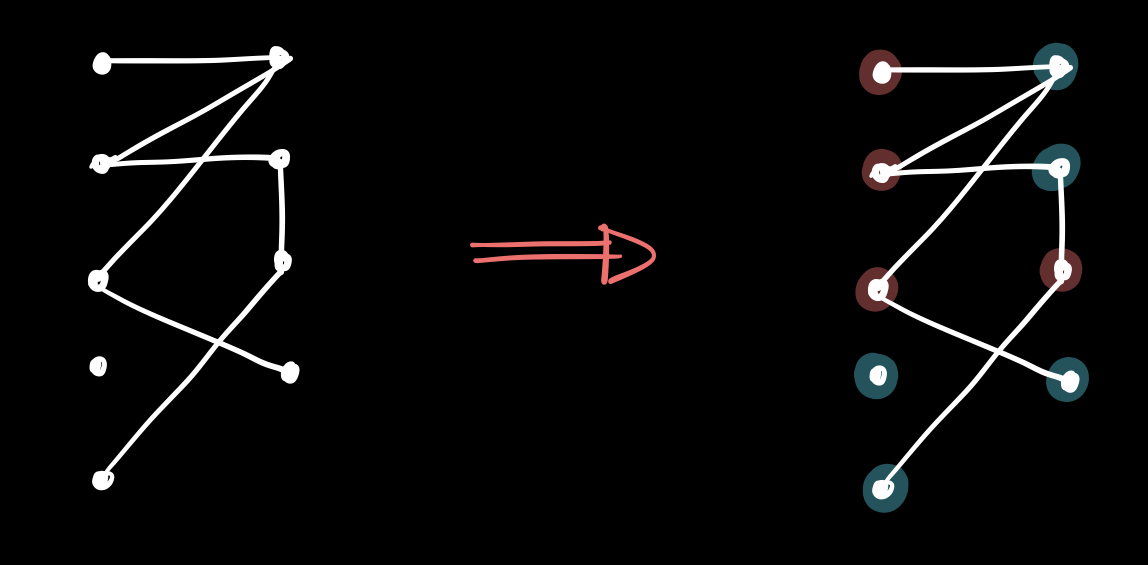
\includegraphics[scale=0.2]{imgs/bipartite.jpeg}
    \caption{Bipartite graph coloring (2-colorable)}
\end{figure}

\end{frame}

\begin{frame}[fragile]
\frametitle{Bipartite Graph Check}

\begin{lstlisting}[language=c]
int s; //initial vertex
queue<int> q; q.push(s);
vector<int> color(V, INF); color[s] = 0;
bool isBipartite = true;

while (!q.empty() && isBipartite) {
	int u = q.front(); q.pop();
	for (auto& v : adjList[u]) {
		if (color[v] == INF){
			color[v] = 1 - color[u]; //two colors {0,1}
			q.push(v);
		} else if (color[v] == color[u]) {
			// Coloring conflict
			isBipartite = false;
			break;
		}
	}
}
\end{lstlisting}

\end{frame}

\begin{frame}[fragile]
\frametitle{Bipartite Graph Check}

\textbf{Example:} \href{https://onlinejudge.org/external/100/10004.pdf}{UVa 10004 - Bicoloring}

\end{frame}

\begin{frame}[fragile]
\frametitle{Graph Edges Property Check via DFS Spanning Tree}

\textbf{Spanning Tree:} given a connected graph $G$, its spanning tree is a tree that spans (covers) all vertices of $G$ but only using a subset of the edges of $G$

\begin{figure}[H]
    \centering
    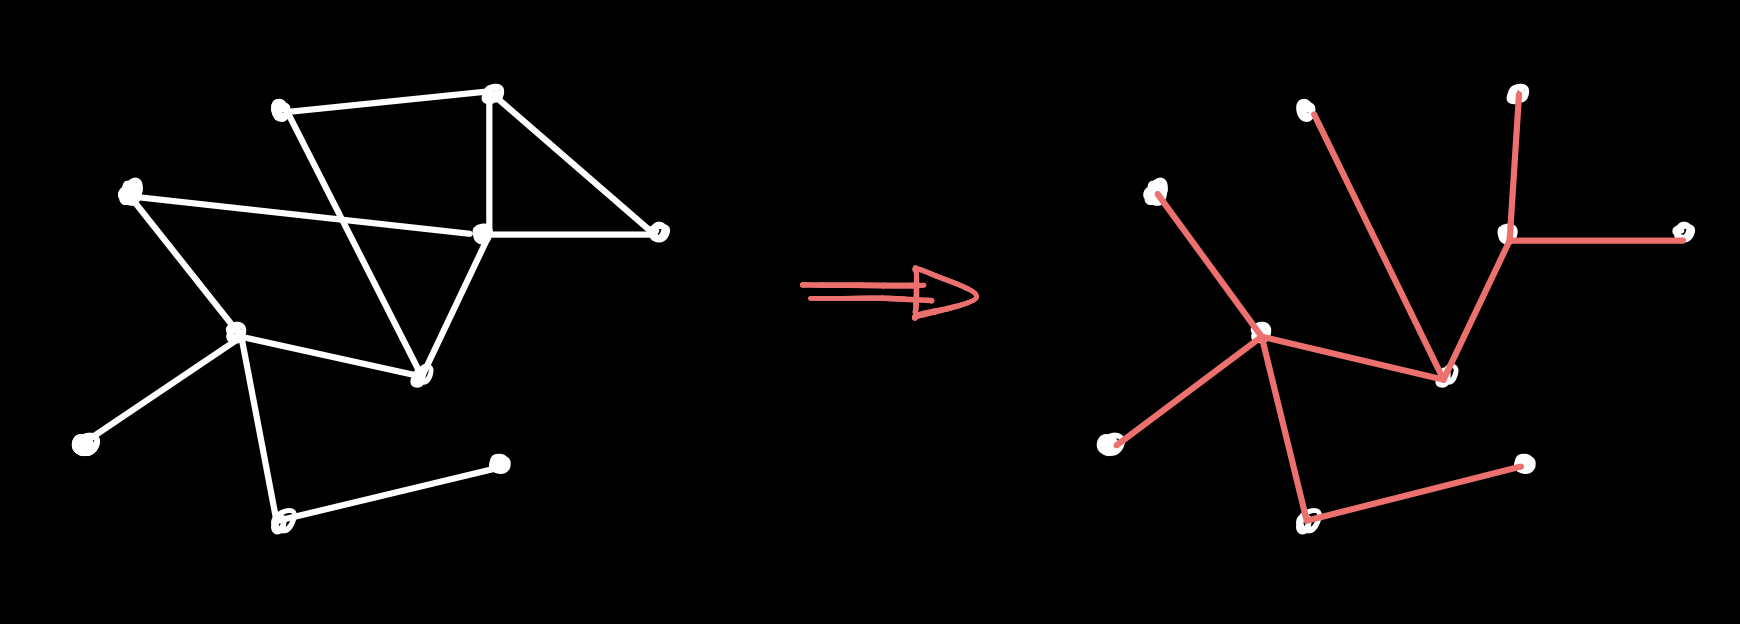
\includegraphics[scale=0.15]{imgs/spanning_tree.jpeg}
    \caption{One possible spanning tree}
\end{figure}

\end{frame}


\begin{frame}[fragile]
\frametitle{Graph Edges Property Check via DFS Spanning Tree}

\begin{itemize}
    \item Running DFS on a connected graph generates a DFS spanning tree
    \pause
    \item We can classify edges into three types using one more vertex state (\verb|EXPLORED| \footnote{EXPLORED: visited but not yet completed} ) in addition to \verb|VISITED| \footnote{VISITED: visited and completed}: 
    	\pause
    	\vspace{0.3cm}
    	\begin{enumerate}
		    \item \textbf{Tree edge}: \verb|EXPLORED| $\rightarrow$ \verb|UNVISITED|. \color{titleColor} -Edge traversed by DFS- \color{fontColor}
		    \pause
		    \item \textbf{Back edge}: \verb|EXPLORED| $\rightarrow$ \verb|EXPLORED|. \color{titleColor} -Edge that is part of a cycle-\color{fontColor}
		    \pause
		    \item \textbf{Forward/Cross edges}: \verb|EXPLORED| $\rightarrow$ \verb|VISITED|
		\end{enumerate}
\end{itemize}

\end{frame}

\begin{frame}[fragile]
\frametitle{Graph Edges Property Check via DFS Spanning Tree}

\begin{figure}[H]
    \centering
    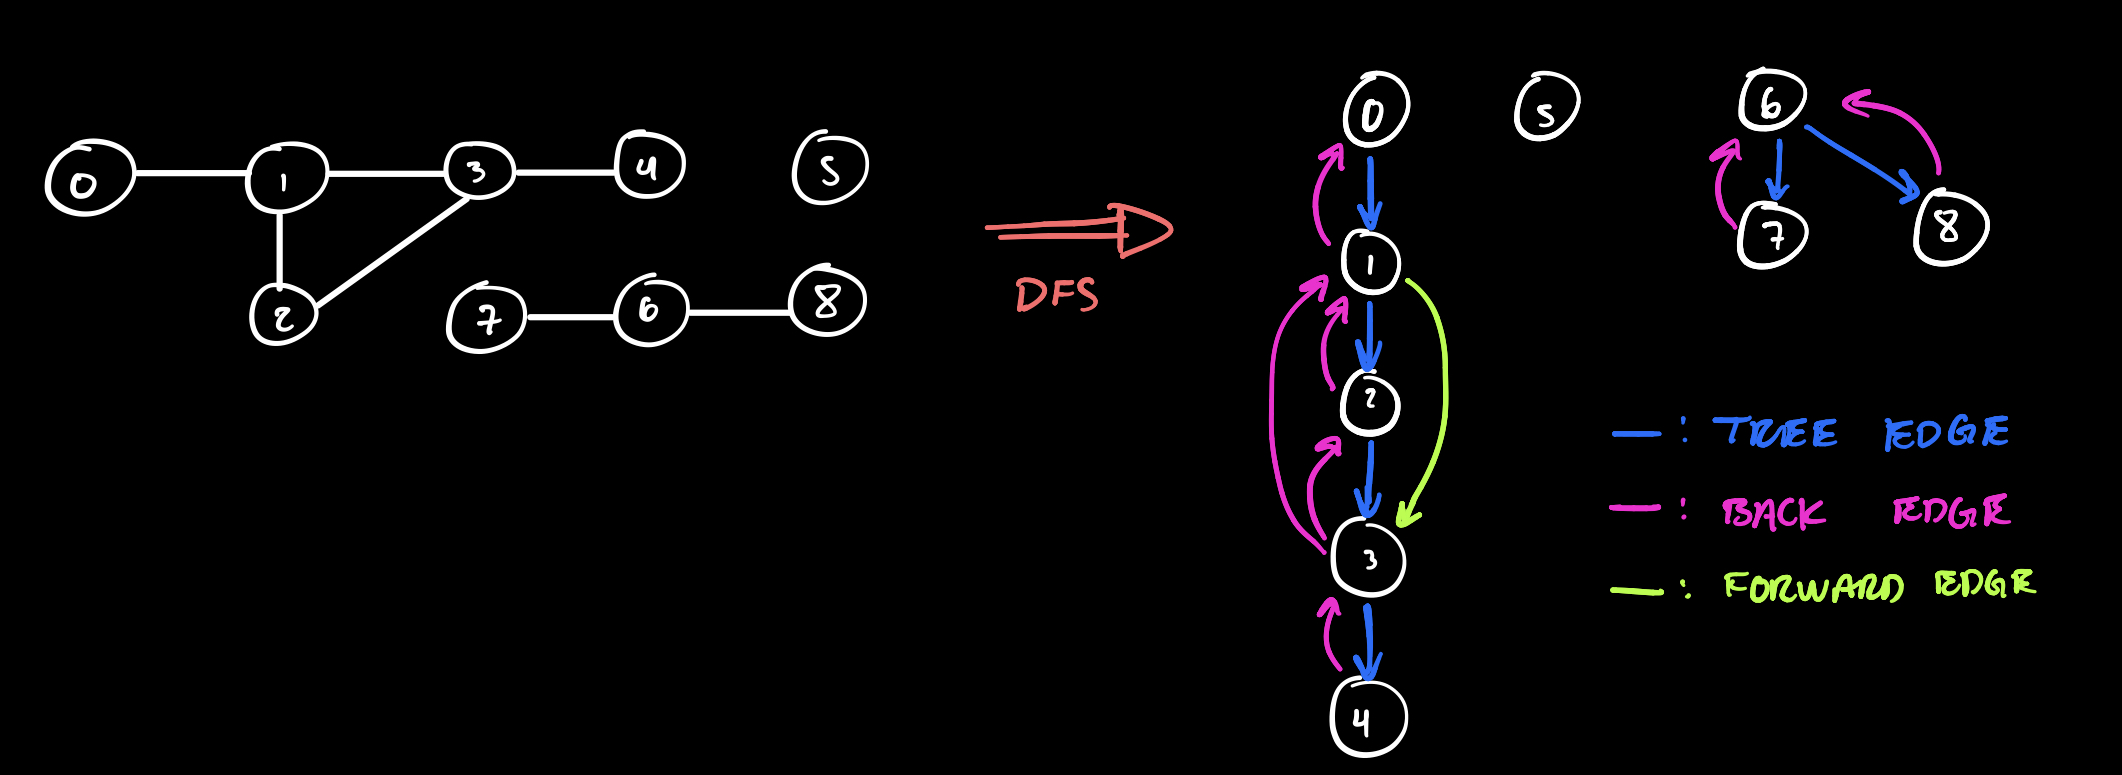
\includegraphics[scale=0.15]{imgs/graph_edge_property_check.jpeg}
    \caption{Example of property check \footnote{An undirected graph with multiple connected components generates a spanning forest}}
\end{figure}

\end{frame}

\begin{frame}[fragile]
\frametitle{Finding Articulation Points and Bridges}

\textbf{Main problem:} Given a road map (undirected graph) with sabotage costs associated to all intersections (vertices) and roads (edges), sabotage either a single intersection or a single road such that the road network breaks down (disconnected) and do so in the least cost way. - \cite{Halim}, p. 130

\end{frame}

\begin{frame}[fragile]
\frametitle{Finding Articulation Points and Bridges}

\begin{itemize}
    \item \textbf{Articulation Point}: vertex in $G$ that its removal will cause $G$ to be disconnected \footnote{A graph without articulation point is called biconnected graph}
    \item \textbf{Bridge}: edge in $G$ that its removal will cause $G$ to become disconnected
\end{itemize}
\pause

\vspace{0.3cm}

\textbf{Note}: these two problems are usually defined for undirected graphs. For directed graphs, they require different algorithms

\end{frame}


%---------------------------------------------------------------------------------------------
%---------------------------------------------------------------------------------------------
%---------------------------------------------------------------------------------------------
\section{4.3 Minimum Spanning Tree}

\begin{frame}[fragile]
\frametitle{Minimum Spanning Tree}

\end{frame}


%---------------------------------------------------------------------------------------------
%---------------------------------------------------------------------------------------------
%---------------------------------------------------------------------------------------------
\section{4.4 Single-Source Shortest Paths}

\begin{frame}[fragile]
\frametitle{Single-Source Shortest Paths}

\end{frame}



%---------------------------------------------------------------------------------------------
%---------------------------------------------------------------------------------------------
%---------------------------------------------------------------------------------------------
\section*{References}
\begin{frame}{References}
    \begin{thebibliography}{}
        \bibitem[Halim]{Halim} Halim S., Halim F., \textit{Competitive Programming 3}, Handbook for ACM ICPC and IOI Contestants. 2013
        \bibitem[Stroustrup]{Stroustrup} Stroustrup B. \textit{The C++ Programming Language}. Fourth ed. 
        \bibitem{skiena} Skiena S. \textit{The Algorithm Design Manual}. Springer. 2020
    \end{thebibliography}
\end{frame}

\end{document}
